\chapter{Test-and-Fallback in Depth}

The test-and-fallback algorithms are the adaptive robustness mechanism
of Chapter 4. This chapter gives their first empirical study in four
parts: the robustness envelope they achieve (§6.1), a counter-intuitive
failure of the acceptance threshold (§6.2), its recalibration (§6.3),
and a benchmark of the dynamic combiner that explains the
\emph{commit-once} structure (§6.4). The resolution limit that
recalibration exposes in §6.3 is this chapter's interface to the
conclusion: it persists across the whole difficulty range, and §10.2
reads it quantitatively. Two naming conventions apply throughout.
FollowPrediction is the unguarded follower, which mimics the advice
matching without testing it; TestAndMatch is the test-and-fallback
scheme in general, of which \textbf{Choo} and \textbf{BEM} are the two
published instantiations. They share the test-then-commit structure and
differ in how the acceptance threshold is set. The \(\ell_1\) test is
the empirical surrogate the original authors also fall back to (Chapter
3).

\section{The robustness envelope}

Sweeping advice error \(\ell_1(p,q)\) on few-types instances (\(n=2000\)
arrivals, \(r=8\) request types, a tested prefix of \(k=200\) arrivals,
40 trials; \textbf{Figure 6.1}), FollowPrediction degrades linearly from
\(1.000\) at perfect advice to \(0.453\) at \(\ell_1\!\approx\!1.1\),
well below the advice-free floor (\(\approx0.99\)). TestAndMatch instead
stays on the \textbf{upper envelope}: it captures the benefit when
advice is good and, when advice is bad, its prefix test rejects it and
it falls back to Ranking, never dropping below the advice-free floor at
any point of this sweep (BEM \(0.998\to0.969\); Choo \(1.000\to0.991\)).
This is the adaptive counterpart of the structural robustness of Chapter
4.

\begin{figure}
\centering
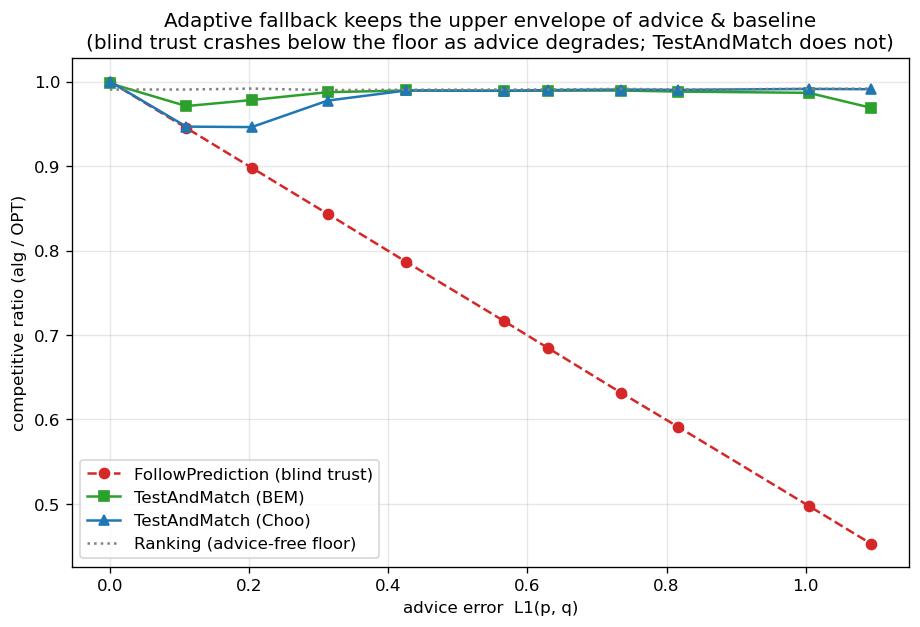
\includegraphics[width=0.5\linewidth,height=\textheight,keepaspectratio,alt={The robustness envelope: blind FollowPrediction crashes below the advice-free floor as advice error grows; TestAndMatch stays on the upper envelope.}]{../../results/choo_bem_envelope.png}
\caption{The robustness envelope: blind FollowPrediction crashes below
the advice-free floor as advice error grows; TestAndMatch stays on the
upper envelope.}
\end{figure}

\section{A threshold that is too lenient on average-case
inputs}

Sweeping the prefix (testing) size \(k\) at \emph{borderline} advice
(\(\eta=0.15\), true \(\ell_1\!\approx\!0.16\)), where the test works
hardest (\textbf{Figure 6.2}), a larger, more accurate test makes the
\emph{worse} decision: as \(k\) grows \(25\to800\), the ratio falls
\(0.992\to0.956\) and the misjudgement rate rises \(0.00\to0.60\).

The mechanism has two halves; the threshold is Choo and BEM's own, and
what follows is our characterization of how it behaves off its design
point. First, the acceptance threshold \(\tau\) is calibrated to
\(\beta\), the competitive ratio the advice-free baseline is
\emph{proved} to achieve: here \(\beta\approx0.696\), Ranking's
worst-case ratio under random arrival order, the value Choo et
al.~instantiate their threshold with \autocite{choo2024imperfect}. On
these instances the realized baseline is instead \(\approx0.99\) (F3),
so the empirical break-even sits at \(\ell_1\approx0\), far below
\(\tau\). Second, the prefix interacts with that gap in opposite
directions at the two ends of the sweep. A small, noisy prefix
over-estimates \(\ell_1\) and rejects the borderline advice, landing
safely on the floor, but it is right for the wrong reason, rejecting
because it is noisy rather than because the advice is bad. A large,
accurate prefix measures \(\ell_1\approx0.16<\tau\) correctly and
therefore accepts the mildly-bad advice that the worst-case threshold
deems acceptable, underperforming the baseline. On strong-baseline
inputs, in other words, the threshold is calibrated against the wrong
baseline, and the size of the prefix decides only how faithfully the
algorithm obeys it.

\begin{figure}
\centering
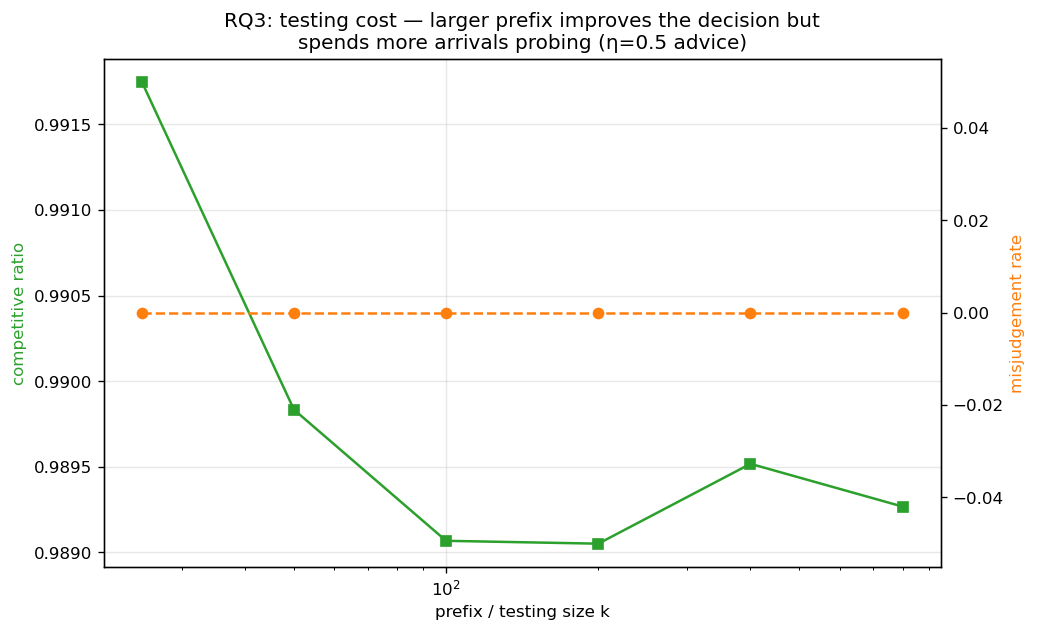
\includegraphics[width=0.5\linewidth,height=\textheight,keepaspectratio,alt={Testing cost at borderline advice: a larger, more accurate prefix test makes the worse decision under the worst-case-calibrated threshold.}]{../../results/choo_bem_prefix.png}
\caption{Testing cost at borderline advice: a larger, more accurate
prefix test makes the \emph{worse} decision under the
worst-case-calibrated threshold.}
\end{figure}

\section{Recalibration, and the resolution limit it
exposes}

By the \textbf{resolution} of a test we mean the smallest difference in
\(\ell_1\) that its empirical estimator can distinguish from its own
sampling noise at prefix length \(k\); this section is about that
quantity and the limit it imposes. Recalibrating \(\tau\) to the
\emph{measured} baseline \(\hat\beta\) eliminates the pathology
(\textbf{Figure 6.3}): at borderline advice the worst-case threshold's
misjudgement climbs \(0.03\to1.00\) as the prefix grows and its ratio
drops to \(0.920\), while the recalibrated threshold holds misjudgement
\(0.00\) at every prefix and ratio \(\approx0.986\). But recalibration
exposes a deeper limit. At perfect advice the worst-case threshold
scores \(1.000\) while the recalibrated one scores only \(0.987\): the
recalibrated \(\tau\approx2(1-\hat\beta)\approx0.028\) is \emph{smaller
than the empirical-\(\ell_1\) estimator's noise floor}: the \(\ell_1\)
distance between a length-\(k\) prefix's type frequencies and the true
histogram under perfect advice, i.e.~pure sampling noise, which falls as
\(k\) grows and spans \(\approx0.13\) down to \(\approx0.05\) over the
prefix lengths swept here, so it can never confidently \emph{accept}: it
rejects everything, including perfect advice, and always plays the
baseline. In short:

\begin{quote}
On strong-baseline instances, among thresholds of this form and at the
prefix lengths we can afford, none both captures the consistency upside
and stays safe: the upside is tiny and sits \emph{below the estimator's
resolution}. The worst-case threshold over-accepts; the recalibrated one
over-rejects; a better tester only follows whichever threshold more
faithfully.
\end{quote}

\begin{figure}
\centering
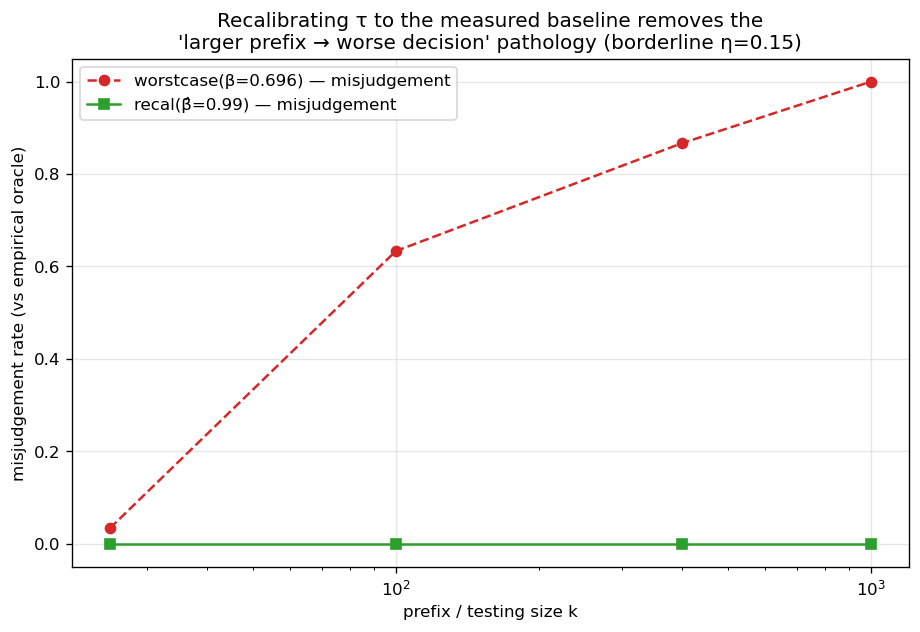
\includegraphics[width=0.5\linewidth,height=\textheight,keepaspectratio,alt={Recalibration removes the threshold pathology: misjudgement holds at zero at every prefix size, versus climbing toward 1.0 under the worst-case threshold.}]{../../results/recalibration_prefix.png}
\caption{Recalibration removes the threshold pathology: misjudgement
holds at zero at every prefix size, versus climbing toward \(1.0\) under
the worst-case threshold.}
\end{figure}

\textbf{Figure 6.4} widens this finding from one threshold to the whole
difficulty range. Sweeping the number of types, the knob that sets the
baseline strength, the \emph{potential} upside of perfect advice grows
as the baseline weakens, but the upside a sublinear-prefix test can
\emph{safely capture} stays pinned near zero: the empirical test's
resolution (its noise floor) sits far above the break-even margin
wherever an upside exists. The wall of this chapter is therefore not one
badly calibrated threshold. The upside and the testing resolution move
together, and the concluding outlook (§10.2) gives this coupling a
quantitative form: the prefix needed to decide scales as the inverse
square of the stakes.

\begin{figure}
\centering
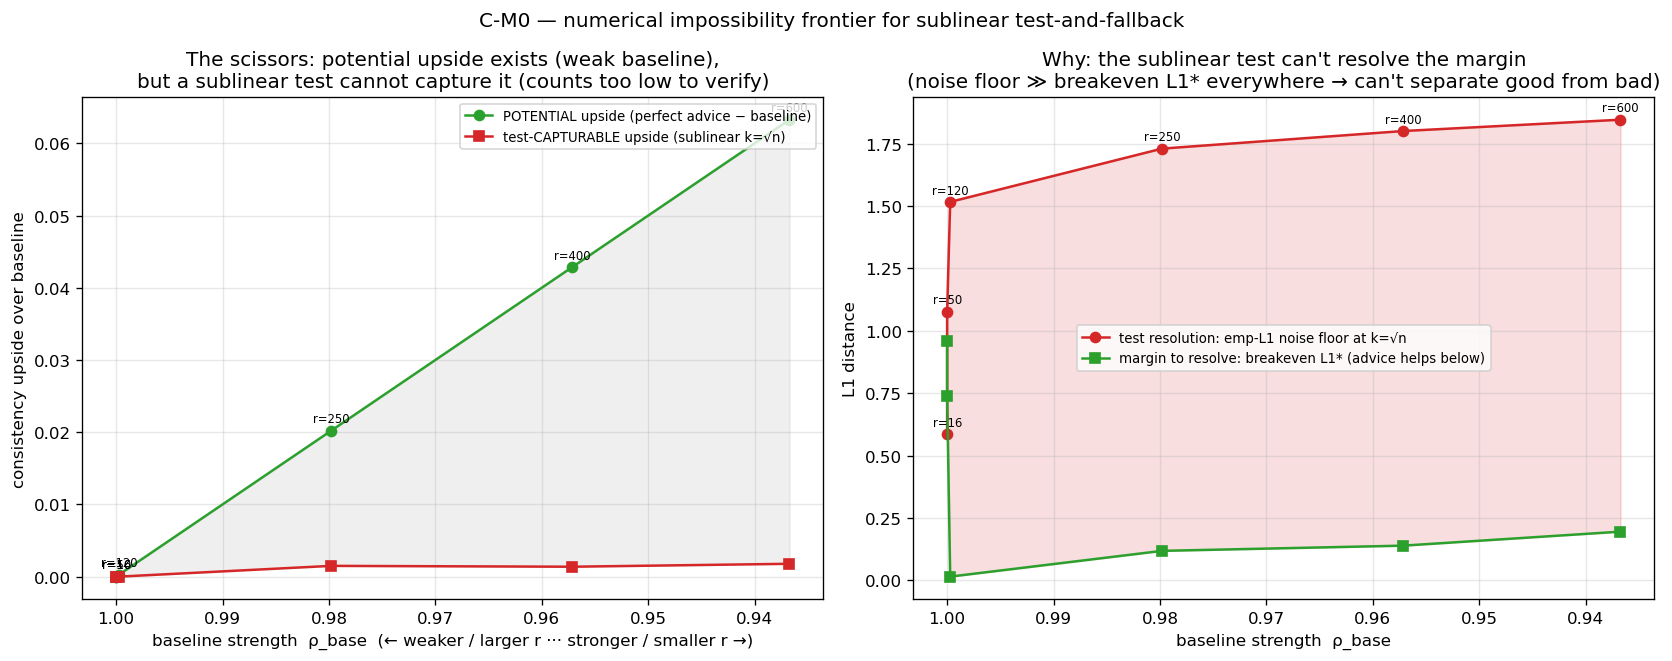
\includegraphics[width=1\linewidth,height=\textheight,keepaspectratio,alt={The testing-wall frontier. Horizontal axis: baseline strength \textbackslash rho\_\{\textbackslash mathrm\{base\}\}, swept by the number of request types (weaker baseline and larger r to the left). Vertical axis: consistency upside over the baseline. As the baseline weakens, the potential upside of perfect advice grows, but the upside captured safely by the sublinear tests examined remains near zero: at the tested points where upside exists, the empirical test's resolution lies above the break-even margin.}]{../../results/impossibility_frontier.png}
\caption{The testing-wall frontier. Horizontal axis: baseline strength
\(\rho_{\mathrm{base}}\), swept by the number of request types (weaker
baseline and larger \(r\) to the left). Vertical axis: consistency
upside over the baseline. As the baseline weakens, the potential upside
of perfect advice grows, but the upside captured safely by the sublinear
tests examined remains near zero: at the tested points where upside
exists, the empirical test's resolution lies above the break-even
margin.}
\end{figure}

\section{The tested dynamic combiner is dominated, illustrating the case
for
test-then-commit}

We benchmark the Chłędowski-style dynamic combiner to contextualize the
commit-once structure of test-and-fallback. In its robust tuning the
combiner sits exactly on the floor of the few-types family of §6.1
(\(0.990\) across all advice quality): it never crashes but captures
none of the consistency upside, strictly dominated by TestAndMatch. More
instructively, an \emph{eager} combiner that switches mid-stream reveals
a penalty specific to irrevocable problems. On a smaller instance used
as a mechanism check (\(n=600\), \(r=6\), a single seed with no
averaging, one of the hand-verifiable scripts of Appendix A.3), eager
switching under perfect advice scores \(0.927\), below both the pure
follower (\(1.000\)) and Ranking on that same instance (\(0.958\)),
because switching from Ranking to advice-following mid-run lands the
committed matching in an \emph{incompatible hybrid}. Being one instance,
this figure illustrates the mechanism rather than measuring its size;
note also that its \(0.958\) is Ranking on that instance, not the
\(0.990\) floor of the family above. In an irrevocable problem the
follow/fallback decision must be made before the bulk of the
commitments, which is why Choo/BEM test a prefix and then commit rather
than switching dynamically. The dynamic combiner that is cheap insurance
for caching does not port cleanly to matching.

\section{Chapter summary}

Test-and-fallback delivers the adaptive robustness envelope of §6.1, but
its accept/reject decision is limited on the strong-baseline inputs
tested here: none of the empirical-\(\ell_1\) thresholds examined both
captures the upside and stays safe (§6.3), and the tested dynamic
switching schemes are dominated by test-then-commit (§6.4). The
resolution limit of §6.3, and its persistence across the tested
difficulty range (Figure 6.4), is the empirical anchor of the
theoretical outlook in §10.2; Figure 6.4 is the figure to remember from
this chapter. The next chapter asks whether any of this survives outside
synthetic instances.
